\documentclass[10pt,twocolumn]{article}
\usepackage{geometry}
\usepackage[utf8]{inputenc}
\usepackage[spanish]{babel}
\usepackage{amsmath} 
\usepackage{cases}
\usepackage{graphicx}

\geometry{margin=0.5in}

%\graphicspath{{./figs/}}

\begin{document}

\author{Nahuel Almeira}

\title{Redes Neuronales 2020\\ FaMAF, UNC\\ Práctico 1}

\maketitle

\section{Introducción}


En este práctico analizaremos el modelo de predadores y presas de Lotka-Volterra. Este modelo es uno de los más icónicos en dinámica de poblaciones, y fue originalmente ideado para modelar una interacción de predación entre dos especies. En nuestro caso, vamos a suponer que las especies en cuestión son zorros (predadores) y conejos (presas), cuyas poblaciones serán representadas por las variables $Z$ y $C$, respectivamente. 

El sistema de Lotka-Volterra se define entonces como el siguiente sistema de ecuaciones diferenciales ordinarias:

\begin{align}
\dot{C} &= \alpha C - \beta C Z \label{eq:LV-C} \\
\dot{Z} &= -\gamma Z + \delta C Z \label{eq:LV-Z},
\end{align}


donde $\alpha$, $\beta$, $\gamma$ y $\delta$ son parámetros reales positivos.

\subsection{Interpretación biológica}

Para interpretar biológicamente los parámetros conviene pensar qué pasaría si cada una de las especies estuviera aislada. En ese caso, tendríamos las siguientes dos ecuaciones no acopladas

\begin{equation}
\dot{C} = \alpha C, \quad \dot{Z} = - \gamma Z.
\end{equation}

Las soluciones a estas ecuaciones son exponenciales. En el caso de los conejos, la población crece exponencialmente, mientras que en el caso de los zorros decrece, tendiendo a la extinción. Cuando una población presenta una variación lineal, como en este caso, la interpretación más simple es considerar que esta variación se debe a una competencia entre el número de nacimientos y el número de muertes. Podríamos pensar entonces que $\alpha = \alpha_N - \alpha_M$, y que $-\gamma = \gamma_N - \gamma_M$, donde los subíndices $N$ y $M$ representan ``nacimientos'' y ``muertes''. Para los conejos, la tasa de natalidad supera a la tasa de mortalidad, por lo que el balance da positivo. En cambio, la mortalidad de los zorros supera a los nacimientos, por lo que el balance da negativo. 

Los parámetros $\beta$ y $\delta$ son propios de la relación interespecífica en cuestión. El primero nos indica la magnitud en la que decrece la cantidad de conejos como producto de la interacción con los zorros (al ser depredados por ellos). El segundo nos indica, de forma análoga, en qué medida se incrementa la cantidad de zorros al depredar a su presa. Es de esperar que $\beta > \delta$ ya que, al ser los zorros una especie más grande que los conejos en términos de biomasa, para incrementar en una unidad la cantidad de zorros, más de un conejo deba ser depredado.


\section{Equilibrios}

Los equilibrios, o puntos fijos del sistema, se definen como los puntos $(C^*,Z^*)^T$ tales que $\dot{C} = \dot{Z} = 0$.

Por inspección, podemos ver fácilmente que el origen es un punto fijo. Para determinar si existen más equilibrios, supongamos $C^* \neq 0$. Luego, de \ref{eq:LV-C} se deduce que $Z^* = \beta / \alpha$. Dado que los parámetros del sistema son todos positivos, deducimos entonces de \ref{eq:LV-Z} que $C^* = \gamma / \delta$. Es decir, los dos únicos puntos fijos del sistema son

\begin{equation}
P_1 =
\begin{bmatrix}
0 \\
0 
\end{bmatrix}
\quad
\text{y}
\quad
P_2 =
\begin{bmatrix}
\gamma / \delta \\
\beta / \alpha
\end{bmatrix}.
\end{equation}



\section{Estabilidad}

Para determinar la estabilidad del sistema, calculamos su matriz jacobiana $A$ y realizamos una linealización del mismo

\begin{equation}
A =
\begin{bmatrix}
\alpha - \beta Z & -\beta C \\
\delta Z & -\gamma + \delta C
\end{bmatrix}
\end{equation}

\subsection{Equilibrio $P_1$}

Evaluando $A$ en el punto $P_1 = (0,0)^T$ obtenemos

\begin{equation}
A =
\begin{bmatrix}
\alpha & 0 \\
0 & -\gamma
\end{bmatrix}.
\end{equation}

La matriz jacobiana es diagonal, y sus autovalores son $\lambda_1 = \alpha > 0$ y $\lambda_2 = -\gamma < 0$. Es decir, se trata de un punto saddle. Los autovectores correspondientes son $v_1 = (1, 0)^T$, correspondiente a la dirección inestable, y $v_2 = (0, 1)^T$, correspondiente a la dirección estable. 

\subsection{Equilibrio $P_2$}

Ahora evaluamos $A$ en el punto $P_2:= (\gamma/\delta, \alpha/\beta)^T$. El resultado es 

\begin{equation}
A =
\begin{bmatrix}
0 & -\dfrac{\beta \gamma}{\delta} \\
\dfrac{\alpha \delta}{\beta} & 0
\end{bmatrix}
\end{equation}

Diagonalizando obtenemos el polinomio característico

\begin{equation}
\lambda^2 + \alpha \gamma = 0.
\end{equation}

Luego, los autovalores son imaginarios puros de la forma $\lambda_{\pm} = i \omega_{\pm}$, con $\omega_{\pm} = \pm \sqrt{\alpha \gamma}$. El hecho de que los autovalores tengan una componente imaginaria indica que las trayectorias cercanas al punto fijo oscilan en torno al mismo. Sin embargo, como la parte real es nula, el criterio no permite determinar la estabilidad del mismo.


\section{Diagrama de flujo}


\begin{figure}[th]
\centering
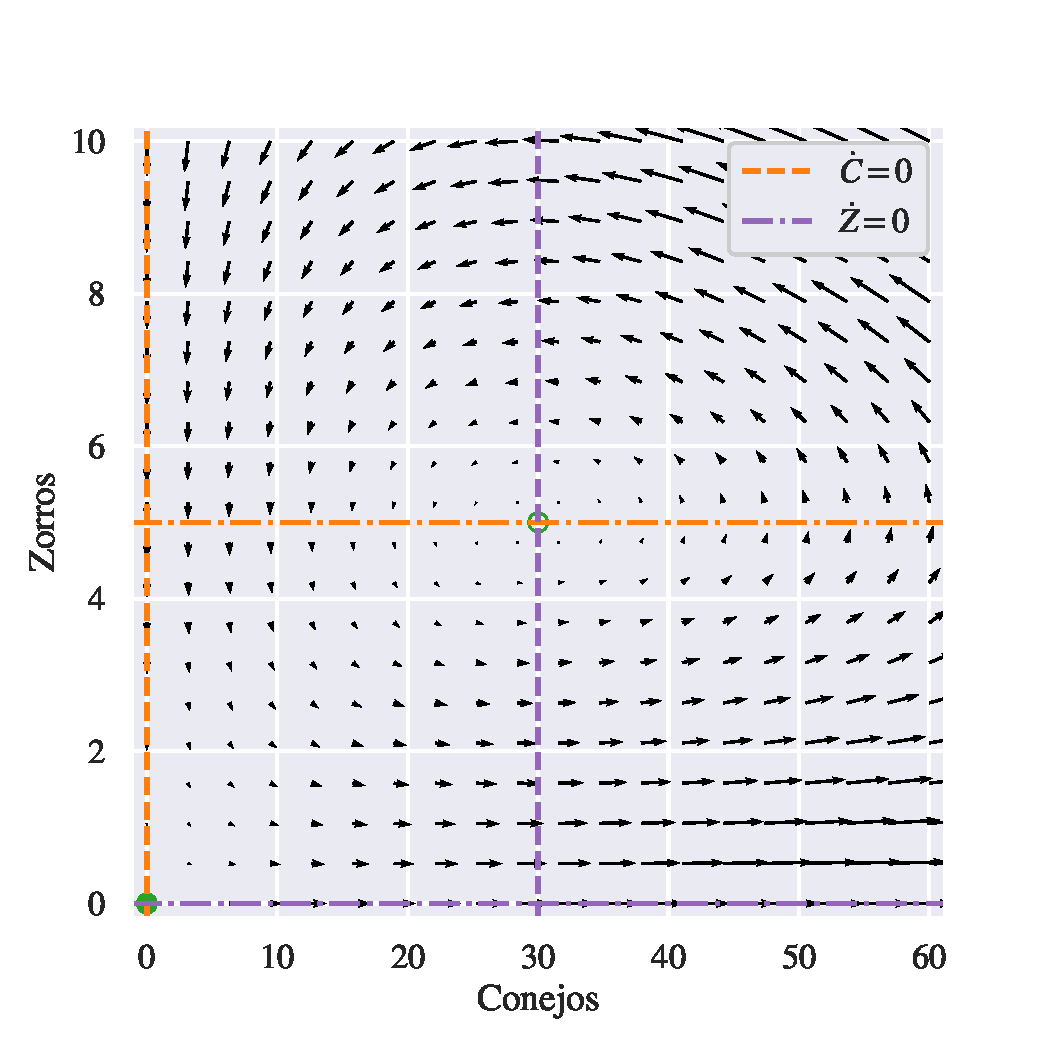
\includegraphics[scale=0.45]{flujo.pdf}
\caption{\label{fig:flujo} Diagrama de flujo del sistema. Los círculos verdes indican los puntos fijos, mientas que las rectas punteadas corresponden a las nullclinas. }
\end{figure}


Para graficar el diagrama de flujo del sistema, nos ayudamos determinando las nullclinas. Es decir, calculamos los puntos del espacio de fase en los que la derivada de alguna de las variables del sistema se anule. Partiendo directamente de \ref{eq:LV-C} y \ref{eq:LV-Z}, podemos ver uqe las nullclinas están descriptas por las curvas


\begin{align}
\dot{C} &= 0\quad  \Rightarrow \quad C = 0 \quad \mathrm{\wedge}\quad Z = \alpha / \beta \\
\dot{Z} &= 0\quad  \Rightarrow \quad Z = 0 \quad \mathrm{\wedge}\quad C = \gamma / \delta 
\end{align}


Además, observando los signos de las derivadas no nulas sobre las nullclinas, podemos determinar que el flujo oscila en torno al equilibrio $E_2$ en dirección antihoraria.

Para continuar analizando el sistema, conviene adimensionalizar las ecuaciones. Para ello, definimos constantes $a$, $b$, $c$, $d$ y $\tau$, y nuevas variables $x$ e $y$ tales que

\begin{equation}
x(t) = \dfrac{\delta C(t)}{\gamma}, \quad y(t) = \dfrac{\beta Z(t)}{\alpha}, \quad \tau = \alpha t, \quad r = \gamma / \alpha.
\end{equation}

Con estas definiciones, podemos reescribir nuestro sistema como 

\begin{equation}
\begin{cases}
\dot{x} &= x (1-y) \\
\dot{y} &= ry (x-1).
\end{cases}
\end{equation}

En el plano de fases adimensionalizado $xy$, las trayectorias están descriptas por las soluciones a la ecuación diferencial

\begin{equation}
\dfrac{dy}{dx} = r\dfrac{y(x-1)}{x(1-y)}.
\end{equation}

Integrando esta ecuación, obtenemos

\begin{equation} \label{eq:energia}
rx + y - \ln x^r y = E,
\end{equation}

con $E = \mathrm{cte}$.
Es decir, el sistema es conservativo y $E$ es la ``energía'', o cantidad conservada, del sistema. Además, podemos ver que el punto $P_2$, que en las nuevas coordenadas es $P_2 = (1,1)$, es un mínimo de la energía. Sabiendo esto, podemos aplicar un teorema (\cite{strogatz}, Teorema 6.5.1), que dice que cualquier trayectoria cercana a $P_2$ es una curva cerrada. En otras palabras, $P_2$ es un centro.



Con esta información, podemos esbozar el diagrama de flujos. En la figura \ref{fig:flujo} mostramos el diagrama, donde las flechas negras indican la dirección e intensidad del flujo en cada punto del espacio. Las nullclinas son representadas mediante rectas punteadas. Los parámetros elegidos fueron $\alpha = 0.1,\; \beta = 0.02,\; \gamma = 0.3,\; \delta = 0.01$.



\section{Evolución temporal}


\begin{figure}[th]
\centering
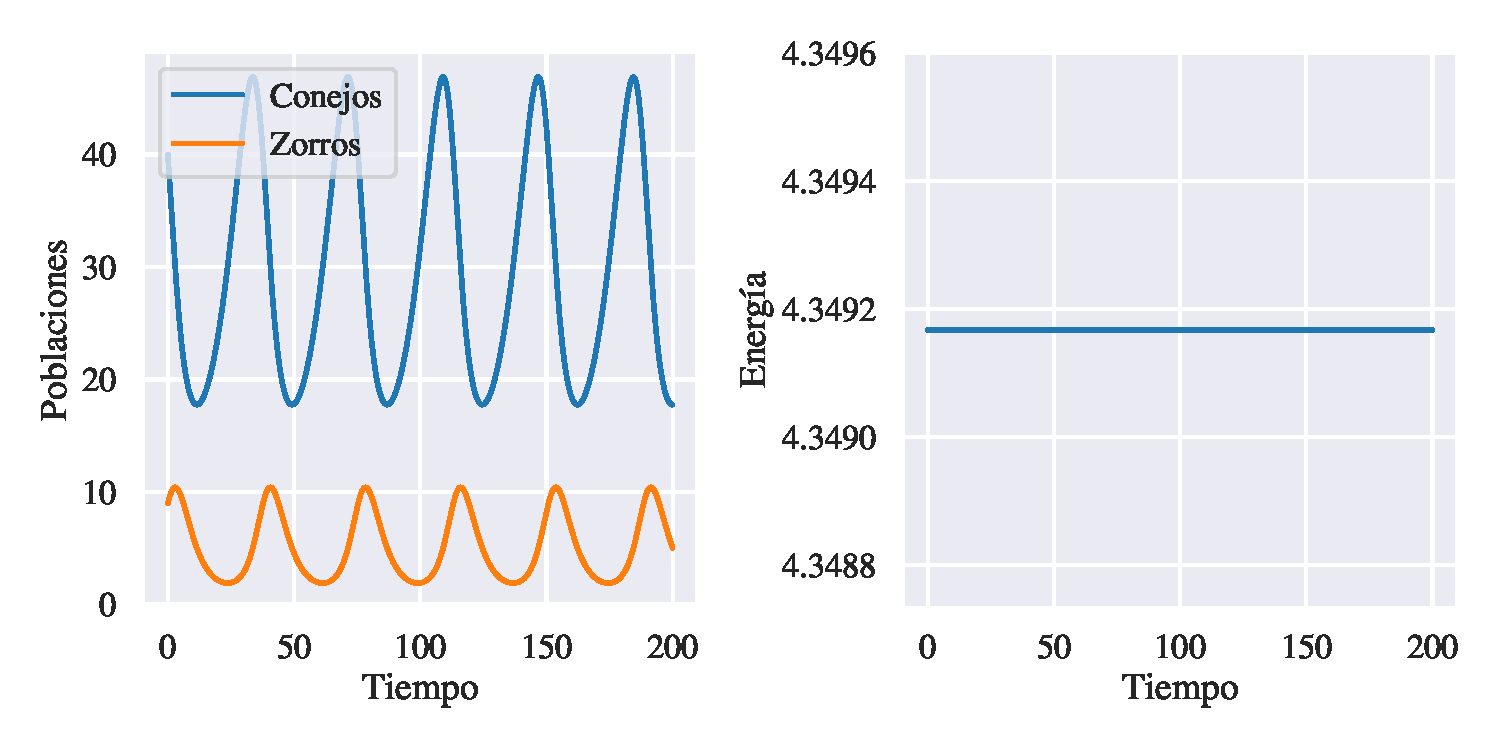
\includegraphics[scale=0.37]{evolucion_y_energia.pdf}
\caption{\label{fig:evolucion} Evolución temporal del sistema. El gráfico de la izquierda muestra el comportamiento de las poblaciones en función del tiempo. Se puede apreciar que las mismas oscilan en forma regular, y que la población de conejos alcanza su pico con anterioridad a la de zorros. En el gráfico de la derecha se muestra la energía del sistema en función del tiempo. El hecho de que se mantenga aproximadamente constante indica que el método de integración empleado no introduce errores numéricos significativos.}
\end{figure}

En esta sección analizamos la evolución temporal del sistema (figura \ref{fig:evolucion}). Para ello, realizamos una integración numérica del sistema mediante el método de Runge-Kutta de cuarto orden con paso $h = 0.05$, en el intervalo temporal $(t_0, t_f) = (0, 200)$. Utilizamos los mismos parámetros que en la sección anterior, y una condición inicial $C(t_0) = 40,\; Z(t_0)=9$. Para corroborar que el método de integración no introduce errores numéricos significativos, calculamos para cada tiempo la energía del sistema, dada por la ecuación \ref{eq:energia}. 



Observamos que ambas poblaciones oscilan de manera estable, en concordancia con la predicción teórica. Además, podemos ver que la población de presa presenta su pico antes que la población de depredadores, lo cual es esperable desde el punto de vista biológico. El gráfico de energía muestra que la misma se conserva durante la integración, indicando que el método empleado, junto con el paso de integración elegido, no introducen un error numérico significativo durante el intervalo de integración.

Como complemento al gráfico de evolución temporal, en la figura \ref{fig:fases} mostramos la trayectoria en el espacio de fases correspondiente a la condición inicial elegida. En este caso, la oscilación se ve como una trayectoria cerrada que encierra al centro $P_2$.

\begin{figure}[t]
\centering
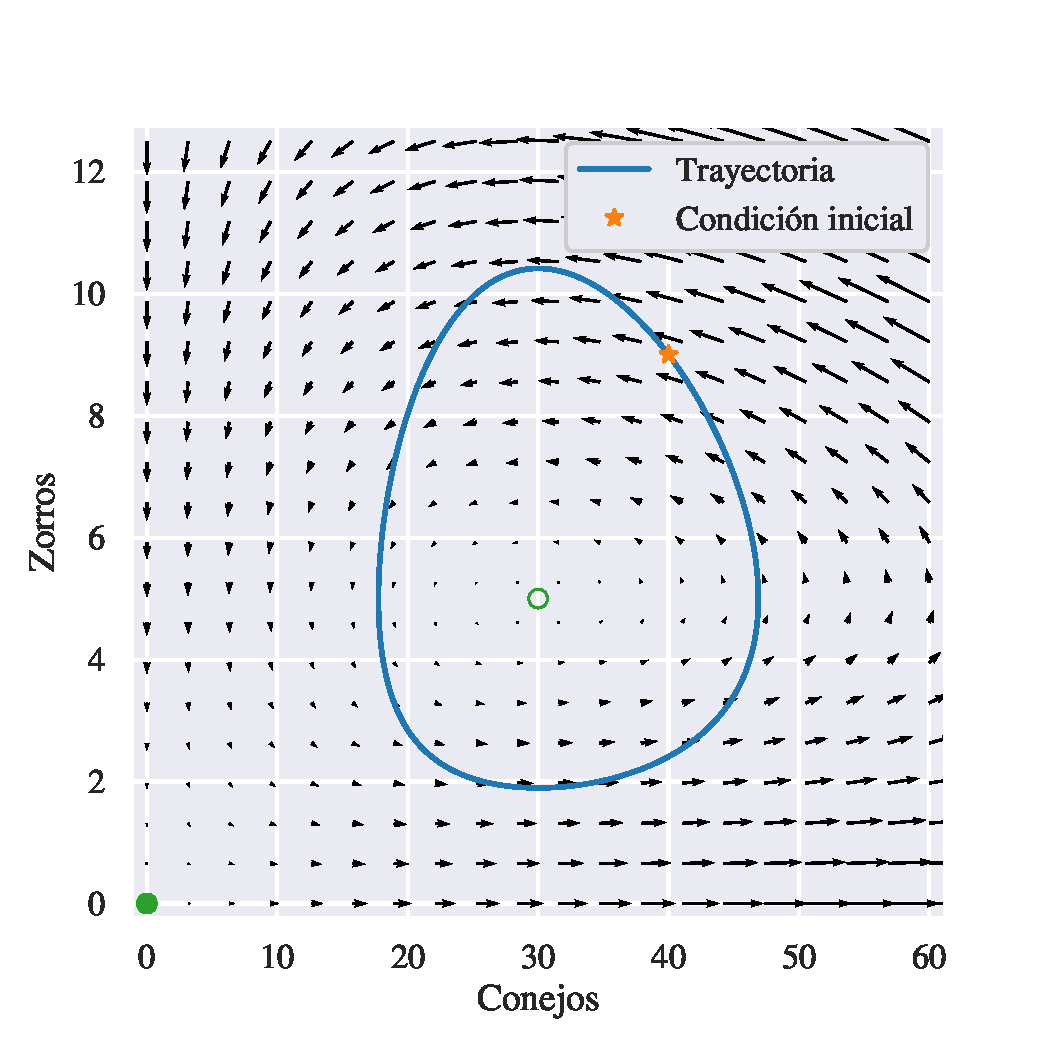
\includegraphics[scale=0.45]{diagrama_de_fases.pdf}
\caption{\label{fig:fases} Trayectoria en el espacio de fases, partiendo de la condición inicial $(C_0, Z_0) = (40, 9)$. }
\end{figure}

\section{Período de oscilación}

\begin{figure}[th]
\centering
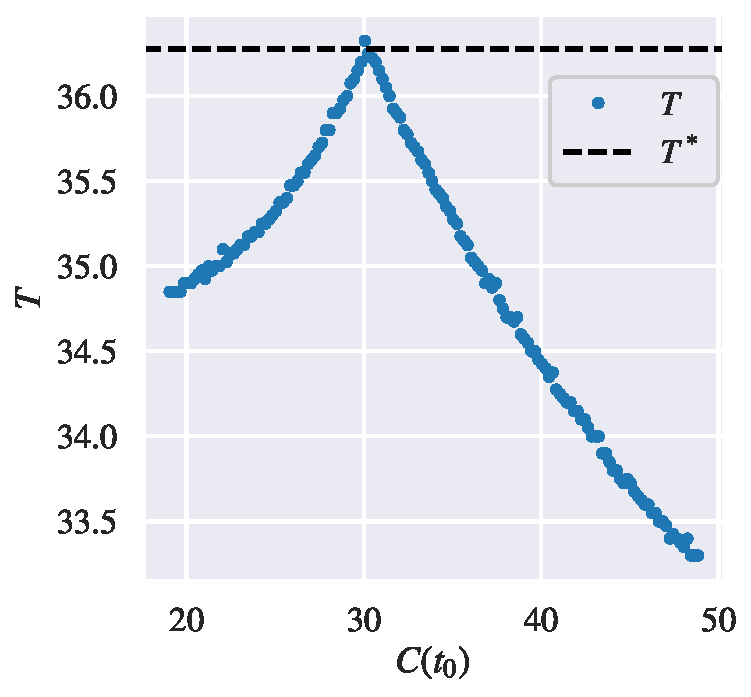
\includegraphics[scale=0.45]{periodo.pdf}
\caption{\label{fig:periodo} 
%Período de oscilación en función de la población inicial de conejos, 
Período de oscilación en función de la población inicial de conejos con población de zorros $Z_0 = 5$. Se observa que el período máximo corresponde a condiciones iniciales cercanas al centro $P_2$. Al alejarse de este punto, las oscilaciones se vuelven más rápidas.}
\end{figure}

%\begin{figure}[ht]
%\centering
%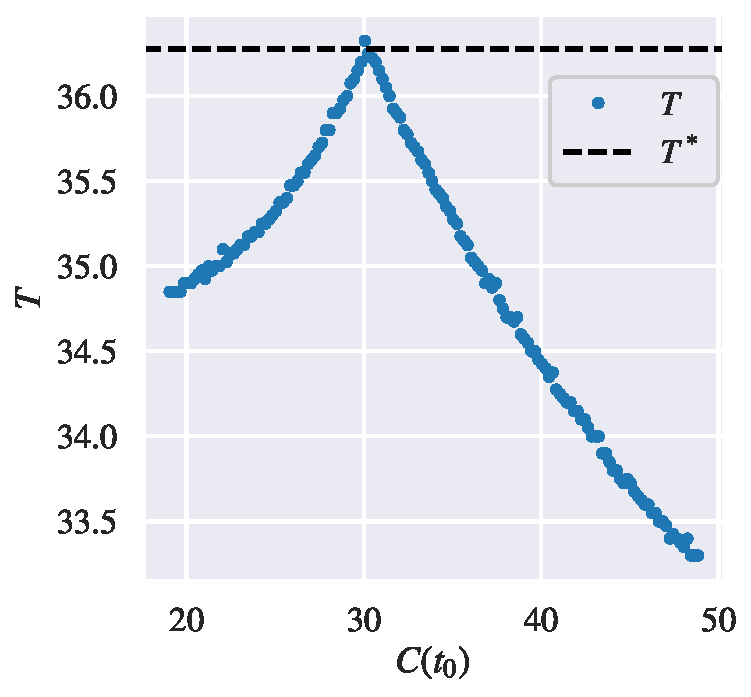
\includegraphics[scale=0.45]{periodo.pdf}
%\caption{\label{fig:_periodo} Período de oscilación en función de la población inicial de conejos, correspondiente a %una población de zorros $Z_0 = 5$. Se observa que el período máximo corresponde a condiciones iniciales cercanas al %centro $P_2$. Al alejarse de este punto, las oscilaciones se vuelven más rápidas.}
%\end{figure}

Desde el punto de vista biológico, resulta interesante analizar el período de las oscilaciones. Para trayectorias que inician en valores cercanos al centro $P_2$, el período puede ser aproximado por $T^* \simeq 2\pi / \omega$, donde $\omega = \sqrt{\alpha \gamma}$ es el valor absoluto de la parte imaginaria de los autovalores $A$ evaluada en $P_2$. 
A medida que la condición inicial se aleje de $P_2$, es esperable que el período varíe, y que la aproximación pierda validez. En la figura \ref{fig:periodo} se puede ver que, al alejarse de la condición inicial, el período disminuye.


\section{Reflexión final}

El modelo de Lokta-Volterra es bueno como una primera aproximación para entender las oscilaciones en especies con interacciones de tipo depredador-presa. Además, dada su simpleza, es posible hacer una interpretación directa de cada uno de sus parámetros en términos biológicos. Sin embargo, el hecho de que el equilibrio de interés sea un centro y que el sistema sea conservativo representa una limitación del sistema, ya que se vuelve sensible a las perturbaciones. Es este sentido, un modelo modificado donde las oscilaciones fuesen producidas por un ciclo límite, sería más realista.


\begin{thebibliography}{9}
\bibitem{strogatz} 
Strogatz, Steven H. Nonlinear Dynamics and Chaos with Applications to Physics, Biology, Chemistry, and Engineering (second edition). CRC Press.
\end{thebibliography}


\end{document}
